% Made up for the tikra benchmark.
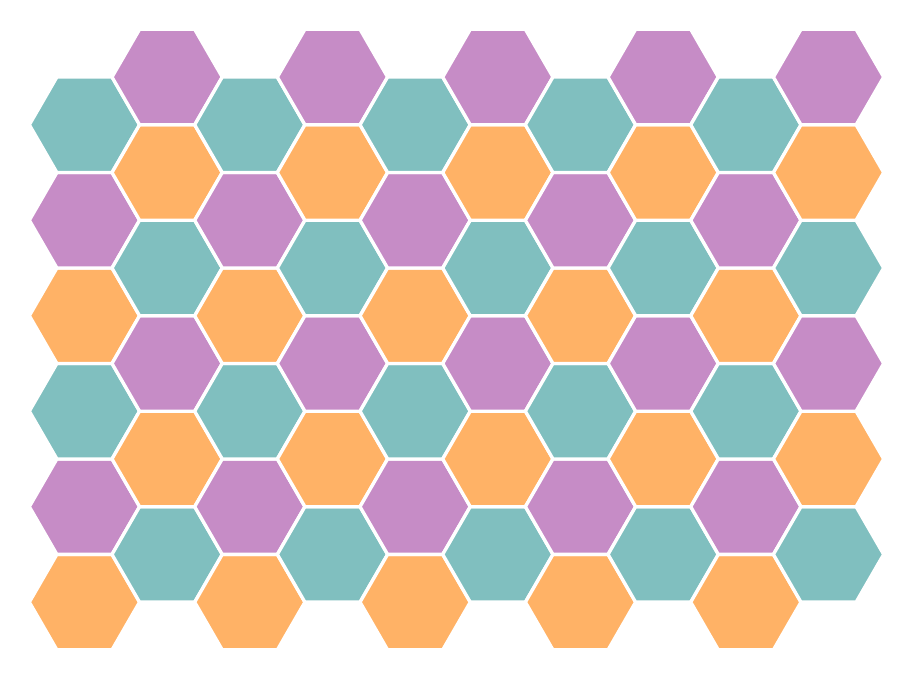
\begin{tikzpicture}[line join=round]
  \colorlet{hex0}{orange!60}
  \colorlet{hex1}{teal!50}
  \colorlet{hex2}{violet!45}
  \def\r{0.7}
  \foreach \i in {0,...,9} {
    \foreach \j in {0,...,5} {
      \pgfmathtruncatemacro\k{mod(30 + \i - \j + floor(\i/2), 3)}
      \pgfmathsetmacro\cx{1.5*\r*\i}
      \pgfmathsetmacro\cy{sqrt(3)*\r*(\j + 0.5*mod(\i,2))}
      \filldraw[fill=hex\k, draw=white, very thick]
        (\cx,\cy) +(0:\r) -- +(60:\r) -- +(120:\r) -- +(180:\r) -- +(240:\r) -- +(300:\r) -- cycle;
    }
  }
\end{tikzpicture}
